
\documentclass[a4paper,10pt]{article}
% This line indicates the type of the document betwin {}: here it is a scientific article.
% Options betwin [] are not mandatory, but precise here:
% - a4paper: printing paper format
% - 10pt: size of the characters

\usepackage{graphicx}
% This package allows to include images
\usepackage{titling}
% This package allows to have a subtitle 
\usepackage{listings}
% this package is used to write code samples.
\lstset{%
  basicstyle=\scriptsize\sffamily,%
  commentstyle=\footnotesize\ttfamily,%
  frameround=trBL,
  frame=single,
  breaklines=true,
  showstringspaces=false,
  numbers=left,
  numberstyle=\tiny,
  numbersep=10pt,
  keywordstyle=\bf
}
\newcommand{\subtitle}[1]{%
  \posttitle{%
    \par\end{center}
    \begin{center}\large#1\end{center}
    \vskip0.5em}%
}



%%%%%%%%%%%%%%%%%%%%%%%%%%%%%%%%%%%%%%%%%%%%%%%%%%%%
% Raport Headers:
%%%%%%%%%%%%%%%%%%%%%%%%%%%%%%%%%%%%%%%%%%%%%%%%%%%%
\title{Image and signal processing: Computer exercise 1}
\subtitle{CE01G02T05}
\author{PRULIERE Valentin \and SID-LAKHDAR Riyane}
\date{26/09/2015}
  
\begin{document}
% Beginning serious stuff. 


\maketitle
% Actually prints title / subtitle / authors and dat into the document


%%%%%%%%%%%%%%%%%%%%%%%%%%%%%%%%%%%%%%%%%%%%%%%%%%%%
% Abstract
%%%%%%%%%%%%%%%%%%%%%%%%%%%%%%%%%%%%%%%%%%%%%%%%%%%%
\begin{abstract}
  This report sumarise, explains and refers to the answers we have designed for the first \"Image and Signal Processing\" computer exercise.\newline 
  Linked to this report you will find \"src/\" directory containing the Python source code corresponding to the exercise' expecations.  
  You will find eather an \"output/\" directory containing some output given by our programs.\newline
\end{abstract}

%%%%%%%%%%%%%%%%%%%%%%%%%%%%%%%%%%%%%%%%%%%%%%%%%%%%
% Introduction
%%%%%%%%%%%%%%%%%%%%%%%%%%%%%%%%%%%%%%%%%%%%%%%%%%%%
\section{Introduction}
The aim of the current computer exercise is to have a first approch with a set of basis theoretical knowledge conserning signal processing.\newline
It eather leads to implement a set of basis programs to create, observe and analyze signal behaviours.\newline
Thus, we have tried to separate as much as possible our theoretical reseaches from the output results.  We have eather tried to implement our programs regardingless to the expected theoretical expectations.\newline
In this purposes, this rapport design tries to respect the convention carried on the given rapport examples.  Thus, the two main sections of this rapport:
  \begin{itemize}
   \item \" Material \& Methods\": In this section, we described the theorical methodes used to answer to every question.  We provide eather the expected algorithms, them main principles, purposes and eventually them implementation in python.
   \item \" Experiments\": In this section, we give the experimental result of our experiences.  We try to explain them, and see whether they are consistant whith the theoretical expecations or not.
  \end{itemize}
Furthermore, to try to make our implementations and results as user frindly as possible the programatic convention we have used is:
  \begin{itemize}
    \item To each python file src/xxx.py corresponds a text file output/xx.txt where the main result of the xx program are stored.
    \item The program names are explicitly linked to the name of the corresponding question, or to the name expected by the question.
    \item The main algorithms which have been implementd are given in the \"Material \& Methods\", and them results are given and described in the \"Experiments\" section.
  \end{itemize}

\section{Material \& Methods}
    \subsection{Exercise 3: Financial Experts}
	\subsubsection{Question 3.1}
	    To create the signal corresponding to the experts prediction, we implemented the file experts.py where we:
	    \begin{itemize}
	    \item Create the signal using its sample values (np.array)
	    \item Plot the signal using the same methodes as in the previous exercise
	    \end{itemize}
	    Our algorithme is given by the following program experts.py
	    \begin{lstlisting}
    import numpy as np
    import matplotlib.pyplot as plt



    # Definition of expertID and expertPrediction tables
    expertID = np.array([1, 2, 3, 4, 5, 6, 7, 8, 9, 10, 11, 12])
    expertPrediction= np.array([996, 868, 855, 956, 867, 933, 866, 887, 936, 901, 818, 956])

    plt.figure()
    line = plt.plot(expertID, expertPrediction, '-', marker='h', linewidth=2)

    plt.grid()
    plt.title('Financial predictions...')
    plt.ylabel('Stock market price prediction')
    plt.xlabel('Financial expert')
    plt.show()

    # Saving the signal
    # Please refer to http://docs.scipy.org/doc/numpy/reference/generated/numpy.savetxt.html
    np.savetxt('../output/experts.txt', (expertID, expertPrediction))
	    \end{lstlisting}

    \subsection{Exercise 4: Mean and Standard Deviation }
	\subsubsection{Question 4.2 \& 4.3}
	    The mean and the standard deviation function has been implemented in the following Python program.
	    \begin{figure}[ht!]
	      \lstset{language=Python}
	      \begin{lstlisting}
    def myMean(signal):
      res = signal[0]
      for k in range(1, len(signal)):
	      res = res + signal[k]
      return res/len(signal)


    def myStandardDeviation(signal):
      mean = myMean(signal)
      s	= 0
      for k in range(len(signal)):
	      s += math.pow((signal[k] - mean),  2)
      return math.sqrt(s / (len(signal)-1))
	      \end{lstlisting}
	      \caption{Python code to compute the mean and the standard deviation of a signal.}
	      \label{ispFunctions_mean_stdDeviation.py}
	    \end{figure}

	\subsubsection{Question 4.4}
	    Laying on the previous algorithms, we can easily compute the mean and the standard deviations of the previous experts signal.</br>
	    The corresponding program is given in the program ispFunctions.py
	    \begin{lstlisting}
    from experts import expertPrediction, trueValue


    mean	= myMean(expertPrediction);
    deviation	= myStandardDeviation(expertPrediction)
    f		= open("../output/ispFunction.txt", 'w')
    f.write("Mean of the experts prediction: " + str(mean))
    f.write("Standard deviation of the experts prediction: "+ str(deviation))
	    \end{lstlisting}

	\subsubsection{Question 4.5}
	    Using the previous programs and the definition of the accuracy, we have implemented the next algorithm to compute the accuracy of a signal.
	    The two last ligns of the program provide the way to use this algorithm to compute the accuracy of the expert's signal.
	    \begin{lstlisting}
      # tv: true average value of the signal (unlike the mean which comes from experimental values)
      def myAccuracy(signal, tv):
	mean = myMean(signal)
	return (math.fabs(tv - mean))
	
      accuracy = myAccuracy(expertPrediction, trueValue)
      f.write("Accuracy of the experts prediction: " + str(accuracy))

	    \end{lstlisting}

    \subsection{Exercise 5: Histogram }
	\subsubsection{Question 5.1 }
	    Given a signal s:
	    \begin{equation} s = \{ x_{0},...,x_{N−1}\}\end{equation}
	    , and a value i that bellongs to [0, N-1].  We know that: \newline
	    \begin{equation} x_{i}\mbox{ counted in }h_{j} \Leftrightarrow\end{equation}
	    \begin{equation} minVal + j*l \leq x_{i} < minVal + (j+1)*l \Leftrightarrow\end{equation}
	    \begin{equation} j*l \leq x_{i} - minVal < (j+1)*l \Leftrightarrow\end{equation}
	    \begin{equation} \mbox{assuming that } l \ne 0: j \leq \frac{x_{i} - minVal}{l} < j+1 \Leftrightarrow\end{equation}
	    \begin{equation} \mbox{Thus, for a given i, } x_{i} \mbox{will be counted in }h_{j}\mbox{ if and only if } j = int(\frac{x_{i} - minVal}{l})\end{equation}

	\subsubsection{Question 5.2 }
	According to the general definition of a histogram, and to the specific purposes described in this question, we can say 
	that the expected histograms of this exercise must show the number of signal samples belonging to each range of value.
	Thus, given a size of values range, our algorithme, will compute the number of diffrent ranges of our histogram (amplitude of the historgam).  
	Then, it will use the previous property to compute the number of signal samples that bellong to this range.   The signal samples are gone through a single time.
	
	\begin{lstlisting}
  def myHistogram(signal,intervalLength):
      minVal = myMin(signal)
      maxVal = myMax(signal)
      length = len(signal)
      N	= int(ceil((maxVal-minVal)/intervalLength)) + 1
      h = [0]*N
      histoAxis = [m * intervalLength + minVal for m in xrange(N)]
      for i in range(0,length - 1):
	      h[int(ceil((signal[i] - minVal)/intervalLength))] += 1

      return h,histoAxis
	 
	\end{lstlisting}


	
    \subsection{Exercise 6: Random signal}
	\subsubsection{Question 6.1 }
	Guiven a random variable X and its corresponding probability function p, we have:
	\begin{equation}E(X) = \int_{-\infty}^{\infty} \! x*p(x) \, \mathrm{d}x \end{equation}
	\begin{equation}     = \int_{-\infty}^{a} \! x*p(x) \, \mathrm{d}x + \int_{a}^{b} \! x*p(x) \, \mathrm{d}x + \int_{b}^{-\infty} \! x*p(x) \, \mathrm{d}x \mbox{according to the Chasles' Theorem} \end{equation}
	We know that the possible values of the variable X bellongs to [a, b].  So p(x) = 0 for each x out of [a, b]. Thus:
	\begin{equation}E(X) = 0 + \int_{a}^{b} \! x*p(x) \, \mathrm{d}x + 0 \end{equation}
	Furthermore, as X is a \textbf{uniformly} random variable, the p function does not depend on its entry x.  Otherwise, the probability that X equals a fixed element from [a, b] is given by the formula:
	\begin{equation} \frac {number of favorable cases}{number of possible case} = \frac{1}{b-a} \mbox{(continuous distribution)}\end{equation}
	Thus, assuming that b and a are diffrents:
	\begin{equation}E(x) = \frac{1}{b-a} * \int_{a}^{b} \! x*p(x) \, \mathrm{d}x\end{equation}
	\begin{equation}     = \frac{1}{b-a} * \frac{b^2 - a^2}{2}\end{equation}
	\begin{equation}     = \frac{b+a}{2} \mbox{which proves the expected property}\end{equation}

	\subsubsection{Question 6.2 }
	To prove the given formula, we will first consider expectation of X square.
	\begin{equation} E(X^2) = \int_a^b \frac{1}{b-a}x^2dx \mbox{ (using the same arguments as in the previous question)}\end{equation}
	\begin{equation}        = \frac{1}{b-a} \int_a^b x^2dx \end{equation}
	\begin{equation}        = \frac{1}{3*(b-a)} (b^3 - a^3) \end{equation}
	\begin{equation}        = \frac{b^2 - ab + a^2}{3} \end{equation}
	thus:
	\begin{equation} \sqrt{E(X)^2 - E(X^2)} = \sqrt{\frac{b^2 - ab + a^2}{3} - \frac{(a+b)^2}{4}}\ \end{equation}
	\begin{equation}                         = \sqrt{\frac{a^2 - 2ab + b^2}{12}} \end{equation}
	\begin{equation}                         = \sqrt{\frac{(a - b)^2}{12}}\ \end{equation}
	thus
	\begin{equation} \sigma_{\chi}            = \frac{(a - b)}{\sqrt{12}}\ \end{equation}

    \subsubsection{Question 6.3 }
    Within this question, we wanted to observe the evolution of the distance between the théorical and the observed values of the mean and the standard deviation.
    Thus we have implemented a program which generates sevral random signals given by them samples.  Each sample size is unique.   Then, for each signal we can:\newline
    \begin{itemize}
     \item Compute the theorical value of the mean and the standard deviation.  This value is given by the previous questions and only depends on the abscissa bounds of the signal.
     \item Compute the measured mean and myStandardDeviation of the signal using the function previously implemented in ispFunctions.py
    \end{itemize}
    Then, for each signal, we keep the ratio of the two mean values, and the ration of the two myStandardDeviation values.\newline
    This algorithm has been implemented in the ispFunction.py file and is shown in the next figure:
    \begin{lstlisting}
#question 6
randomSignalSize= np.array([10000, 20000, 30000, 40000, 50000, 60000, 70000, 80000, 90000, 100000])
meanDistance	= np.array(range(0, size(randomSignalSize)), dtype=float)
stdDeviationDistance= np.array(range(0, size(randomSignalSize)), dtype=float)
for i in range(0, size(randomSignalSize)):
    signal	= np.random.random(randomSignalSize[i])
    mean	= myMean(signal)
    deviation	= myStandardDeviation(signal)
    a  		= 0
    b		= randomSignalSize[i]-1
    meanDistance[i]		= 10*mean	/ ((a+b)/2)
    stdDeviationDistance[i]	= deviation	/ ((b-a)/math.sqrt(12))


plt.figure()
line = plt.plot(randomSignalSize, meanDistance, '--', color='blue', linewidth=2)
line = plt.plot(randomSignalSize, stdDeviationDistance, '-', color='red', linewidth=2)

plt.grid()
plt.title('Theoretical VS computed values...')
plt.xlabel('Number of sample by signal')
plt.ylabel('Ratio of the theoretical and the computed value')
plt.show()
    \end{lstlisting}

    In the 10th line of the algorithm, we can see that the distance between theorical and measured value of the mean is multipyed by 10 for each signal.
    This 10 coefficient is used to make the corresponding plot more user frindly.  
    Thus, the corresponding plot will bee in the same values range as the standard deviation distance plot.  
    This coefficient does not change the increasing or decreasing character of the distance function.

    \subsubsection{Question 6.4 }
    The probability distribution function of a random variable X bellonging to [a, b] is known as:\newline
    \begin{equation}\chi:  [a, b]  \to [0, 1] \end{equation}
    \begin{equation}  x       \mapsto p(\chi < x)\mbox{ : the probability that X be lower than x} \end{equation}
    Thus, for an equiprobable random variable X, \begin{equation}p(\chi<x) = \frac{x - a}{b - a}  \end{equation}
    Secondly, we know by the definition that the probability density function of a random variable is its derivte over x (x represents its single variable).\newline
    So the probability density function F of an equiprobable random variable is:
    \begin{equation} F(x) = \frac{1}{b-a}\end{equation}
    Assuming that a = 0, and b = 1, we have
    \begin{equation} F(x) = 1\end{equation}


\section{Experiments}
    \subsection{Exercise 2: Signal Storage and Display Example}
	\subsubsection{Question 2.1}
	    The given program gives a partial definition of a signal (given by a sample of some of its values).  It eather shows how to plot it using simple python graphical librarys.
	    The output plot of this program is given by the figure \ref{exampleSignalFigure}:
	    \begin{figure}[ht!]
	      \center
	      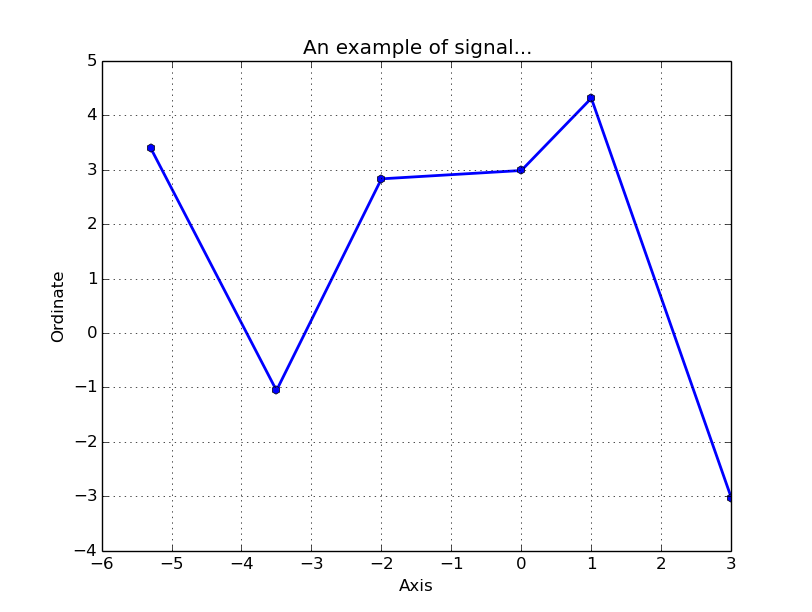
\includegraphics[width=0.8\linewidth]{exampleSignal.png}
	      \caption{Example of a sample signal plot realised in a python}
	      \label{exampleSignalFigure}
	    \end{figure}

    \subsection{Exercise 3: Financial Experts}
	\subsubsection{Question 3.1}
	    Our program (desribed in the material and methods sections) allowed us to plot the signal corresponding to the expert predictions.  This output plot is given by the figure: \ref{expertsSignalFigure}.
	    \begin{figure}[ht!]
	      \center
	      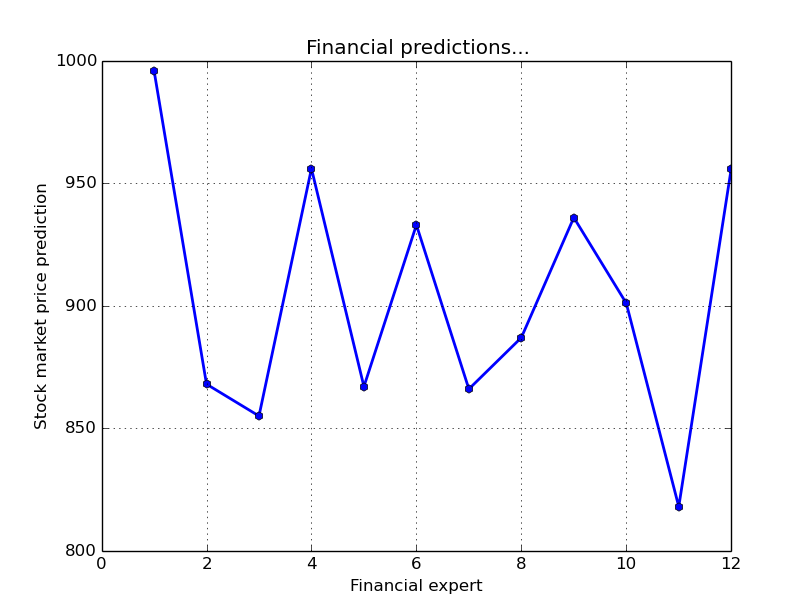
\includegraphics[width=0.8\linewidth]{expertsSignal.png}
	      \caption{Expert's signal plot}
	      \label{expertsSignalFigure}
	    \end{figure}

    \subsection{Exercise 4: Mean and Standard Deviation }
	\subsubsection{Question 4.4 \& 4.5}
	Using the program described in the \"Material \& Methods\" section, we have computed the following values for the experts signal:
	\begin{itemize}
	\item Mean of the experts prediction: 903
	\item Standard deviation of the experts prediction: 52.1666908704
	\item Accuracy of the experts prediction: 27.0
	\end{itemize}
	
	
    \subsection{Exercise 6: Random signal}
    \subsubsection{Question 6.3 }
	The figur \ref{theoreticalVScomputed} has been obtained by runing the algorithm described in the algorithm of the section 2.4.3.\newline
	The figure represents the evolution over the signal samples size of the ration of:
	\begin{itemize}
	 \item Theoretical and measured values of the mean of the signal: blue broken  curve
	 \item Theoretical and measured values of the standard deviation of the signal: red continue curve
	\end{itemize}

	\begin{figure}[ht!]
	  \center
	  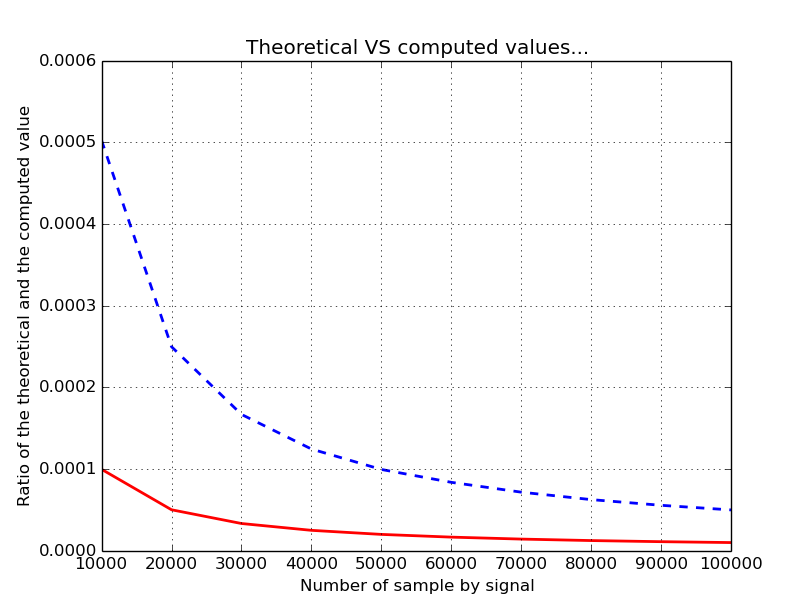
\includegraphics[width=0.8\linewidth]{theoreticalVScomputed.png}
	  \caption{Evolution of the ration of the thoretical and measured values of the mean and the standard deviation}
	  \label{theoreticalVScomputed}
	\end{figure}
	This plot illustrates the fact that the mor samples we generate, the closer the measured mean and standard deviation get to the theoretical mathematical expectation and standard deviation of the underlying random variable.
	
	


\section{Conclusion}
This current rapport trys to summerise the experiments we have been dealing with durring this first computer exercise.  It analyzes the experimental results and explains whether they sute or not the theoretical expectations.\newline
During this practical sessions, we have eather ben able to develope some functionality for signal visualization and processing. However the developed algorithms seem verry simple, they may already give an intresting vision about some signal behaviours.
\end{document}
